\chapter{Metodologia}\label{cap:metodologia}

Este capítulo operacionaliza o problema de pesquisa delimitado nos capítulos anteriores: comparar a capacidade de ferramentas SAST tradicionais, de agentes empresariais de codificação baseados em IA e de uma abordagem híbrida SAST + IA para detectar, explicar e priorizar vulnerabilidades em aplicações Python. A fundamentação e os critérios de escolha de Bandit, Semgrep Community Edition, Cursor e OpenAI Codex foram apresentados no Capítulo~\ref{cap:fundTeoric}; neste capítulo, o foco recai sobre como essas ferramentas foram executadas sobre o benchmark RealVuln, quais dados foram coletados e como os resultados foram avaliados. O protocolo foi definido antes da coleta; quando a execução se afastou do planejado, o desvio é indicado nesta seção e detalhado na Seção~\ref{sec:desvios-protocolo}.

A metodologia adota um desenho empírico comparativo, com medidas repetidas sobre os mesmos repositórios Python e o \textit{ground truth} público e versionado do RealVuln \cite{Pellew2026RealVuln}. Um repositório controlador organizou a versão fixada do benchmark, as cópias entregues às ferramentas, as instruções e os resultados, mantendo os arquivos de resposta fora do alcance dos agentes durante a análise. Bandit e Semgrep foram invocados pelo \textit{harness} em contêineres Docker efêmeros e equivalentes. As ferramentas empresariais de IA foram avaliadas sobre o mesmo código sanitizado, com instruções, permissões e recursos controlados.

\section{Questões de Pesquisa}\label{sec:questoes-pesquisa-metodologia}

O experimento é orientado pelas seguintes questões de pesquisa:

\begin{enumerate}
\item[\textbf{QP1}] Qual é o desempenho de cada condição experimental na detecção de vulnerabilidades Python, considerando precisão, \textit{recall}, F1, F2, F3 e taxa de falsos positivos?
\item[\textbf{QP2}] Qual é a qualidade dos relatórios verdadeiros-positivos quanto à correção técnica, localização, clareza e acionabilidade?
\item[\textbf{QP3}] Em que medida fornecer os alertas de Bandit e Semgrep aos agentes de IA melhora ou degrada a detecção e a qualidade dos relatórios em relação às ferramentas executadas isoladamente?
\item[\textbf{QP4}] Quão estáveis são os resultados das condições baseadas em IA entre execuções independentes e quão adequadamente essas condições indicam a prioridade dos achados quando existe uma referência de severidade confiável?
\end{enumerate}

As QP1 e QP3 constituem o eixo quantitativo principal. A QP2 acrescenta a avaliação da utilidade prática dos relatórios, enquanto a QP4 combina medidas quantitativas de estabilidade e concordância com a análise da priorização, dimensões apontadas como pouco exploradas pela literatura revisada \cite{Germano2025LLMSLR, Mao2025ExplainableVD, Tamberg2025LLMHarness}. O tempo de execução e o consumo de tokens são apresentados como caracterização operacional complementar, sem constituir uma questão de pesquisa autônoma.

As questões não compartilham a mesma base: a QP1 usa todas as execuções sobre as 817 entradas, enquanto a QP2 se restringe a uma amostra de relatos verdadeiros-positivos. A QP3 reaproveita as medidas das QP1 e QP2, mas compara cada condição híbrida com a condição isolada do mesmo produto sobre os mesmos projetos.

\section{Classificação e Desenho da Pesquisa}\label{sec:classificacao-pesquisa}

Quanto à natureza, a pesquisa é aplicada, pois produz evidência empírica destinada a apoiar a escolha e a combinação de ferramentas de análise de segurança no ecossistema Python. Quanto à abordagem, emprega métodos mistos com predominância quantitativa: as condições são comparadas por métricas derivadas da matriz de confusão, enquanto a qualidade dos relatórios é examinada por uma rubrica estruturada. Quanto aos objetivos, o estudo é exploratório e descritivo-comparativo. Não se pretende demonstrar causalidade geral sobre todas as ferramentas ou modelos de IA, mas caracterizar diferenças observadas sob as condições controladas deste protocolo.

O procedimento central é um experimento computacional de medidas repetidas: cada condição experimental é aplicada aos mesmos repositórios da versão fixada do RealVuln. A comparação utiliza as vulnerabilidades e os falsos-positivos armadilha já rotulados pelo benchmark, reduzindo a influência de diferenças de corpus entre as ferramentas. A pesquisa bibliográfica apresentada nos capítulos anteriores fundamenta a escolha das condições, dos dados, das métricas e das ameaças à validade; o desenvolvimento do \textit{harness} constitui a instrumentação necessária para integrar Cursor e Codex ao formato de resultados e ao avaliador do benchmark.

\section{Condições Experimentais}\label{sec:condicoes-experimentais}

As três abordagens conceituais do trabalho são operacionalizadas em seis condições, apresentadas na Tabela~\ref{tab:condicoes-experimentais}. Bandit e Semgrep são avaliados separadamente, conforme suas diferenças técnicas discutidas na Seção~\ref{subsec:ferramentas-sast}. Cursor e Codex também permanecem separados, evitando que uma união artificial de suas respostas seja interpretada como uma única ferramenta. No braço híbrido, a união normalizada e sem duplicatas dos alertas de Bandit e Semgrep é fornecida, como contexto adicional, a uma nova execução de cada agente.

\begin{table}[htb]
\ABNTEXfontereduzida
\caption{\label{tab:condicoes-experimentais}Condições experimentais avaliadas}
\centering
\begin{tabularx}{\textwidth}{|l|X|X|}
\hline
\textbf{Condição} & \textbf{Execução} & \textbf{Papel na comparação} \\
\hline
C1 & Bandit em configuração fixada & Linha de base SAST específica para Python \\
\hline
C2 & Semgrep Community Edition com conjunto de regras fixado & Linha de base SAST baseada em regras declarativas \\
\hline
C3 & Cursor com GPT-5.6 Luna, sem receber alertas SAST & Agente empresarial isolado com modelo controlado \\
\hline
C4 & OpenAI Codex com GPT-5.6 Luna, sem receber alertas SAST & Agente empresarial isolado com modelo controlado \\
\hline
C5 & Alertas normalizados de C1 e C2 fornecidos ao Cursor com GPT-5.6 Luna & Condição híbrida SAST $\rightarrow$ Cursor com modelo controlado \\
\hline
C6 & Alertas normalizados de C1 e C2 fornecidos ao Codex com GPT-5.6 Luna & Condição híbrida SAST $\rightarrow$ Codex com modelo controlado \\
\hline
\end{tabularx}
\legend{Fonte: Elaborado pelo autor (2026).}
\end{table}

A Figura~\ref{fig:desenho-experimental} apresenta o desenho experimental completo. As três faixas correspondem às abordagens comparadas e recebem o mesmo código sanitizado. Os alertas de C1 e C2 são unidos e entregues, sem alteração, às duas condições híbridas. O \textit{ground truth} permanece do outro lado da barreira de cegamento e só é usado na avaliação, depois do fechamento da coleta.

\begin{figure}[htbp]
\centering
\caption{\label{fig:desenho-experimental}Desenho experimental: corpus, condições, controles e avaliação}
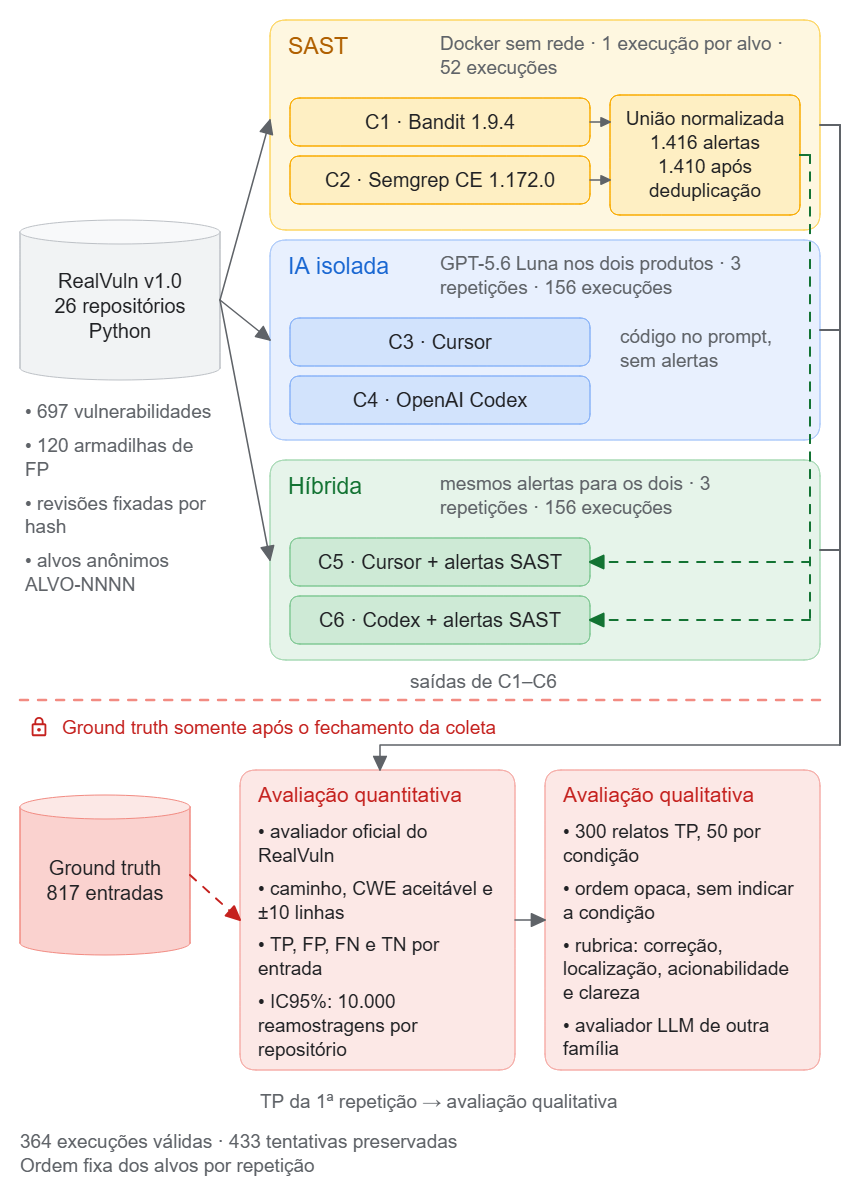
\includegraphics[width=0.96\textwidth]{figs/excalidraw/metodologia-desenho-experimental-legivel.png}
\legend{Fonte: Elaborado pelo autor (2026).}
\end{figure}

Os resultados primários são reportados por condição, e não apenas agregados nos rótulos ``SAST'', ``IA'' e ``híbrido''. Sínteses por abordagem aparecem apenas como leitura complementar, preservando os valores individuais e sem tratar ferramentas diferentes como observações independentes de uma população de ferramentas.

O bloco experimental principal utilizou o GPT-5.6 Luna em C3--C6. A adoção do mesmo modelo reduz o confundimento entre a capacidade do modelo subjacente e os efeitos próprios da ferramenta, como seleção de contexto, orquestração e interface. O identificador do modelo, o nível de raciocínio, o modo de contexto e as demais opções observáveis foram fixados no estudo-piloto e mantidos durante todo o bloco \cite{Cursor2026Models, OpenAI2026ModelGuidance}.

O planejamento admitia um bloco complementar com as configurações nativas indicadas pelos fornecedores: o modo Auto no Cursor e o GPT-5.6 Terra no Codex. O Auto é uma estratégia adaptativa de seleção e pode encaminhar solicitações a modelos diferentes; por isso, não seria tratado como equivalente ao Terra nem combinado com a linha de base Luna. A regra definida antes da coleta previa executar esse bloco somente se as cotas comportassem o corpus completo, com as mesmas três repetições, evitando uma seleção posterior de repositórios favoráveis. O bloco complementar não foi executado, e os resultados deste trabalho restringem-se ao bloco Luna.

Nas condições C3 e C4, os agentes não puderam executar Bandit, Semgrep ou outros analisadores de segurança. Nas condições C5 e C6, receberam os alertas SAST previamente coletados, sem acesso ao \textit{ground truth}. Para garantir que os dois produtos recebessem exatamente o mesmo material, o código Python sanitizado de cada alvo foi enviado no próprio \textit{prompt}, e a escrita de arquivos, a execução de comandos e o acesso à rede foram restringidos da forma mais equivalente permitida pelos dois produtos, conforme a Seção~\ref{subsec:adaptadores-sessao-ia}. Com isso, a característica agêntica de navegação autônoma pelo repositório, discutida na Seção~\ref{sec:agentes-codificacao}, não foi avaliada.

\section{Universo, Corpus e Unidade de Análise}\label{sec:universo-amostra}

O universo de interesse compreende vulnerabilidades classificáveis por CWE em projetos Python. O corpus experimental foi a versão 1.0 do RealVuln descrita por \citeonline{Pellew2026RealVuln}, composta por 26 repositórios Python intencionalmente vulneráveis e 817 entradas: 697 vulnerabilidades e 120 armadilhas. Essa versão foi usada integralmente, caracterizando um censo do \textit{release} escolhido, e não uma nova amostra construída pelo autor.

A escolha do RealVuln decorre de sua correspondência direta com o objetivo do trabalho: o benchmark foi projetado para comparar ferramentas baseadas em regras e scanners baseados em LLM sobre os mesmos repositórios, publica o código-fonte, o \textit{ground truth}, o algoritmo de correspondência e os scripts de pontuação, além de incluir exemplos seguros necessários ao cálculo de falsos positivos \cite{Pellew2026RealVuln}. O VUDENC permanece relevante como evidência histórica sobre detecção em Python, mas não foi adotado como corpus deste experimento porque sua rotulagem automática e sua granularidade em janelas de tokens exigiriam uma reconstrução de \textit{ground truth} incompatível com a comparação em nível de repositório.

A unidade de análise é a entrada rotulada do RealVuln: uma vulnerabilidade conhecida ou um falso-positivo armadilha, associada a repositório, arquivo, intervalo de linhas, CWE e evidência. A unidade de execução é um repositório completo analisado por uma condição experimental. A unidade de observação é o achado individual emitido pela condição, posteriormente associado, ou não, a uma entrada do \textit{ground truth}. Essa distinção mantém o projeto inteiro como objeto de análise, sem reduzir a avaliação a funções isoladas.

Foram fixados o identificador da versão do benchmark, o \textit{commit} do repositório RealVuln, o \textit{commit} de cada projeto-alvo e o \textit{hash} dos arquivos de \textit{ground truth}. Nenhum repositório ou rótulo foi removido após a observação dos resultados. Para uma falha técnica que impedisse uma condição de concluir um projeto, previu-se o modo estrito do benchmark: as vulnerabilidades daquele projeto seriam contabilizadas como não detectadas, e a falha, reportada separadamente.

\section{Controle do Corpus e Cegamento}\label{sec:repositorio-experimental}

O RealVuln não foi alterado nem teve suas vulnerabilidades recriadas. Para cada repositório, utilizou-se a revisão indicada pelo manifesto oficial, e as seis condições receberam o mesmo conteúdo verificável por \textit{hash}. Código-fonte, configurações, dependências declaradas e testes pertencentes à revisão foram preservados; metadados de versionamento, artefatos gerados e documentos que revelassem explicitamente as respostas foram excluídos por uma regra definida antes da coleta e aplicada de forma idêntica a todas as condições.

O \textit{ground truth}, o avaliador e a correspondência entre os projetos originais e seus identificadores opacos permaneceram fisicamente separados das áreas entregues às ferramentas. Cada execução utilizou uma área de trabalho nova. As condições de IA receberam apenas o código e a instrução padronizada; nas condições híbridas, acrescentou-se somente a união normalizada dos alertas de C1 e C2, sem indicação de verdadeiro ou falso positivo. Esses controles reduzem a exposição direta das respostas e evitam estado residual entre condições e repetições.

Um manifesto interno registrou o alvo, a condição, a repetição, o \textit{commit}, o \textit{hash} da entrada e o estado da execução. Ele permitiu retomar a fila após interrupções sem reutilizar áreas de trabalho ou sessões anteriores. A estrutura de diretórios e os mecanismos utilizados para implementar essa separação são descritos no Capítulo~\ref{cap:desenvolvimento}, Seção~\ref{sec:organizacao-repositorio-desenvolvimento}.

\section{Importação e Uso do \textit{Ground Truth}}\label{sec:ground-truth-metodologia}

O \textit{ground truth} foi importado diretamente da versão fixada do RealVuln, sem reconstrução ou alteração de rótulos pelo autor. Cada entrada contém identificador, indicação de vulnerabilidade ou armadilha segura, CWE principal, conjunto de CWEs aceitáveis, arquivo, intervalo de linhas, severidade e evidência de rotulagem \cite{Pellew2026RealVuln}. Antes da coleta, o arquivo foi validado pelo verificador disponibilizado pelo benchmark e seu \textit{hash}, registrado.

Preservou-se o algoritmo de correspondência do benchmark: caminho de arquivo normalizado, CWE pertencente ao conjunto aceitável da entrada e linha dentro da tolerância definida pelo RealVuln. Cada entrada pode ser consumida uma única vez, evitando que alertas duplicados ampliem artificialmente a detecção. As saídas de Bandit, Semgrep, Cursor e Codex foram apenas convertidas para o esquema de entrada esperado pelo avaliador; a lógica de pontuação não foi reimplementada, pois o script oficial pôde ser reutilizado.

Conforme as regras do RealVuln, um achado associado a uma entrada vulnerável é verdadeiro positivo; um achado associado a uma armadilha segura ou não associado a nenhuma entrada é falso positivo; uma vulnerabilidade sem correspondência é falso negativo; e uma armadilha corretamente ignorada é verdadeiro negativo. Os rótulos não foram corrigidos durante a coleta, e não foi realizada análise de sensibilidade com rótulos alterados; todos os resultados usam a versão oficial.

Cada achado percorre três verificações sucessivas: arquivo, CWE aceitável e linha dentro da faixa rotulada com tolerância de dez linhas. Basta uma resposta negativa para o achado ser contado como falso positivo sem correspondência, o que explica por que um alerta tecnicamente plausível, mas com CWE fora do conjunto aceitável ou linha deslocada, reduz a precisão. Quando há correspondência, a natureza da entrada decide entre verdadeiro positivo e falso positivo em armadilha, e a entrada é consumida. Só depois de processados todos os achados, as entradas restantes tornam-se falsos negativos ou verdadeiros negativos.

\section{Ambiente de Execução e Docker}\label{sec:materiais-ambiente}

A Tabela~\ref{tab:ambiente-experimental} apresenta os principais materiais e controles do ambiente. A justificativa técnica das ferramentas foi desenvolvida no Capítulo~\ref{cap:fundTeoric}; aqui são registrados apenas os elementos necessários à reprodução das execuções.

\begin{table}[htb]
\ABNTEXfontereduzida
\caption{\label{tab:ambiente-experimental}Materiais e controles do ambiente experimental}
\centering
\begin{tabularx}{\textwidth}{|l|X|X|}
\hline
\textbf{Categoria} & \textbf{Item} & \textbf{Controle registrado} \\
\hline
SAST & Bandit & Versão, comando, configuração, imagem Docker, duração e saída JSON \\
\hline
SAST & Semgrep Community Edition & Versão, comando, regras locais, \textit{hash} das regras, imagem Docker, duração e saída JSON \\
\hline
Conteinerização & Docker & Versão do motor, imagem-base por \textit{digest}, limites de recursos, rede e volumes \\
\hline
IA empresarial & Cursor & Versão do cliente, estratégia de seleção, modelo solicitado e efetivamente exibido, nível de raciocínio, modo de contexto, data e hora, instrução, permissões, duração, consumo de tokens informado e identificador da sessão \\
\hline
IA empresarial & OpenAI Codex & Versão do cliente, modelo solicitado e efetivamente exibido, nível de raciocínio, modo de contexto, data e hora, instrução, permissões, duração, consumo de tokens informado e identificador da sessão \\
\hline
Dados & RealVuln v1.0 & 26 repositórios, manifesto, 817 entradas rotuladas, \textit{ground truth} e avaliador fixados por \textit{hash} \\
\hline
Infraestrutura & \textit{Harness} em Python & Código versionado, esquema comum, registros brutos, normalização e cálculo das métricas \\
\hline
\end{tabularx}
\legend{Fonte: Elaborado pelo autor (2026).}
\end{table}

Bandit e Semgrep foram executados a partir de uma imagem Docker imutável, com versões fixadas, código-alvo somente para leitura e saída gravada separadamente. Cada combinação entre ferramenta e repositório utilizou um contêiner novo, sem rede, com usuário sem privilégios e os mesmos limites de CPU, memória e tempo. Assim, a conteinerização atua como variável de controle das condições SAST, enquanto o manifesto externo ao contêiner permite retomar a fila de execuções.

Em conformidade com a delimitação estabelecida na Seção~\ref{subsec:ferramentas-sast}, não foram criadas regras específicas para os repositórios do corpus. O Bandit foi executado com seu conjunto nativo de \textit{plugins} e sem supressões ajustadas após a observação dos resultados. O Semgrep Community Edition utilizou um conjunto público de regras de segurança para Python, selecionado antes do estudo-piloto, copiado para \texttt{docker/regras-semgrep/} e fixado por versão e \textit{hash}. O nome do conjunto, os arquivos efetivamente carregados e a linha de comando completa foram publicados, pois a expressão ``configuração padrão'' não identifica sozinha quais regras públicas foram aplicadas pelo Semgrep.

A conteinerização equaliza o ambiente local das condições C1 e C2, mas não torna os serviços de IA equivalentes nem imutáveis. Por isso, cada condição de C3--C6 foi executada em uma janela de coleta tão curta quanto possível, com sessões novas, o mesmo texto de instrução, o mesmo código e permissões equivalentes, e o modelo foi fixado em GPT-5.6 Luna nos dois produtos. Previu-se interromper e reiniciar, ou analisar separadamente, um bloco afetado por alteração de modelo ou de produto durante a coleta; as versões efetivamente observadas estão na Seção~\ref{sec:registro-configuracao-desenvolvimento}. A construção da imagem, os comandos e os adaptadores pertencem à implementação e são detalhados no Capítulo~\ref{cap:desenvolvimento}.

\section{Instrumentação e Dados Coletados}\label{subsec:implementacao-harness}

Um \textit{harness} em Python e PowerShell foi utilizado para preparar entradas idênticas, controlar a fila, preservar saídas brutas e metadados e converter os achados para o formato aceito pelo avaliador. Para cada execução foram registrados, no mínimo, condição, ferramenta, bloco de modelos, alvo, repetição, arquivo, intervalo de linhas, regra ou CWE informado, severidade, descrição, recomendação, duração e estado da execução. Nas condições baseadas em IA, foram registrados também a estratégia de seleção, o modelo solicitado, o modelo efetivamente exibido e os consumos de tokens de entrada, de saída e total quando esses dados foram disponibilizados pelo produto.

As condições C3--C6 deveriam emitir uma lista JSON com caminho do arquivo, linha inicial e final, CWE, severidade, descrição da causa e recomendação. A lista vazia era aceita como ausência de achados. Campos omitidos permaneceram nulos: o normalizador não utilizou o \textit{ground truth} para completar localizações, CWE ou severidades. A união SAST fornecida às condições híbridas foi deduplicada antes da nova execução dos agentes, mantendo a origem dos alertas e sem anexar rótulos do benchmark.

Os adaptadores foram verificados antes da coleta com saídas artificiais externas ao corpus e com uma execução de fumaça descartável. A arquitetura do \textit{harness}, o esquema comum, as regras de deduplicação, os comandos e os testes de integração são especificados no Capítulo~\ref{cap:desenvolvimento}, Seções~\ref{sec:arquitetura-harness} e~\ref{sec:verificacao-artefato-desenvolvimento}.

\section{Métricas de Avaliação}\label{sec:metricas-metodologia}

\subsection{Métricas quantitativas de detecção}\label{subsec:metricas-quantitativas-metodologia}

A matriz de confusão foi produzida pelo avaliador do RealVuln no nível das entradas rotuladas. Vulnerabilidades correspondidas são verdadeiros positivos (TP), vulnerabilidades não encontradas são falsos negativos (FN), armadilhas ou regiões não rotuladas sinalizadas são falsos positivos (FP), e armadilhas corretamente ignoradas são verdadeiros negativos (TN). A pontuação principal utilizou o modo estrito e agregado por microcontagem do benchmark, no qual uma falha completa de análise não é removida do denominador \cite{Pellew2026RealVuln}.

Foram calculadas, por condição, repositório, categoria CWE e severidade:

\begin{itemize}
\item \textbf{Precisão}: $TP/(TP+FP)$;
\item \textbf{Recall}: $TP/(TP+FN)$;
\item \textbf{F1}: média harmônica entre precisão e \textit{recall};
\item \textbf{F2}: média harmônica ponderada com maior peso para o \textit{recall}, adequada à maior criticidade dos falsos negativos em segurança \cite{Kalouptsoglou2023VulnPrediction};
\item \textbf{F3}: média harmônica ponderada que atribui peso nove vezes maior ao \textit{recall}, métrica principal do RealVuln \cite{Pellew2026RealVuln};
\item \textbf{Taxa de falsos positivos}: $FP/(FP+TN)$.
\end{itemize}

A leitura das medidas de detecção considera sua direção: precisão, \textit{recall}, F1, F2 e F3 maiores indicam melhor desempenho segundo seus respectivos critérios; uma taxa de falsos positivos menor indica menos alertas incorretos em relação ao denominador adotado pelo benchmark. Precisão e \textit{recall} respondem a perguntas diferentes: a primeira mede quantos alertas emitidos estão corretos, e o segundo mede quantas vulnerabilidades existentes foram encontradas. Uma ferramenta pode, portanto, apresentar precisão alta e deixar muitas falhas sem detecção. A análise por CWE e severidade é apresentada mesmo quando a quantidade de entradas permitir apenas interpretação descritiva.

\subsubsection{Intervalo de confiança de 95\% e comparações pareadas}\label{subsubsec:ic95-metodologia}

O intervalo de confiança de 95\% (IC95\%) acompanha a estimativa pontual para expressar sua incerteza diante da composição dos projetos. O ponto resume o resultado observado; os dois limites mostram uma faixa obtida pelo procedimento de reamostragem. Um intervalo mais amplo indica maior incerteza. O nível de 95\% se refere à cobertura esperada do procedimento em amostragens repetidas sob seus pressupostos: não significa que a ferramenta acerta 95\% das vulnerabilidades, nem atribui uma probabilidade de 95\% ao parâmetro depois de calculado o intervalo.

O cálculo utiliza \textit{bootstrap} percentil no nível do repositório, implementado em \path{runner/avaliacao/estatistica.py}, com 10.000 reamostragens e semente 20260928. Em cada reamostragem, são sorteados 26 projetos com reposição: um mesmo projeto pode aparecer mais de uma vez, e outro pode não aparecer. Todas as entradas e repetições de um projeto são mantidas juntas. Esse agrupamento evita tratar as vulnerabilidades de um mesmo repositório como observações independentes.

Para cada conjunto sorteado, somam-se TP, FP, FN e TN e recalculam-se as métricas. Em C1 e C2, utiliza-se a execução única; em C3--C6, calcula-se a métrica separadamente em cada uma das três repetições e toma-se sua média. Não se unem os achados das repetições. Os percentis 2,5 e 97,5 das 10.000 estimativas definem, respectivamente, os limites inferior e superior do IC95\%.

Por exemplo, um F3 de 18,6\% com IC95\% de 14,8\% a 22,4\% indica a estimativa observada e a incerteza calculada por esse procedimento. Nos gráficos, o marcador representa o ponto e as hastes representam os limites. Esses intervalos caracterizam a sensibilidade à composição dos 26 projetos; não garantem desempenho em produção e não abrangem toda a variabilidade de futuras respostas dos modelos.

As comparações híbrida--isolada são pareadas: C5 e C3, assim como C6 e C4, recebem exatamente o mesmo conjunto sorteado de projetos em cada reamostragem. A diferença é definida como híbrida menos isolada. Para precisão, \textit{recall} e F3, diferenças positivas favorecem a condição híbrida; para a taxa de falsos positivos, diferenças negativas a favorecem. As diferenças são expressas em pontos percentuais: passar de 25\% a 28\% corresponde a três pontos percentuais.

O IC95\% da diferença é obtido pelos mesmos percentis. Se ele incluir zero, os dados não estabelecem uma direção de vantagem pelo critério adotado, pois o intervalo admite tanto ausência de diferença quanto valores favoráveis a condições distintas. Isso não prova equivalência. A decisão utiliza o intervalo da diferença pareada, e não apenas a sobreposição dos intervalos individuais. Os escores qualitativos e seus contrastes no recorte comum permanecem descritivos, sem IC95\% ou inferência de superioridade.

Em cada reamostragem dos 26 projetos do corpus, projetos podem ser sorteados mais de uma vez, ocupando o lugar daqueles que ficaram de fora. Cada reamostragem produz uma estimativa, e os percentis 2,5 e 97,5 da distribuição das 10.000 estimativas delimitam o IC95\%. Como a condição híbrida e a isolada são calculadas sobre a mesma reamostragem, ambas usam a mesma composição de projetos em cada sorteio, e a decisão depende de o intervalo da diferença incluir ou não o zero.

\subsection{Tempo de execução e consumo de tokens}\label{subsec:tempo-tokens-metodologia}

O tempo de execução foi medido pelo \textit{harness} como tempo de relógio entre o envio da tarefa e a disponibilidade da saída final. Nas condições SAST, registrou-se também a duração do processo do analisador. Nas condições de IA, o tempo compreende a chamada ao agente até sua resposta final ou até o limite de execução previamente definido. São reportados mediana, intervalo interquartil e valores mínimos e máximos por condição, pois tempos de serviços remotos podem apresentar distribuição assimétrica.

O consumo de tokens foi coletado apenas nas condições baseadas em IA e conforme os contadores efetivamente disponibilizados por cada produto. Foram preservados separadamente tokens de entrada, tokens de saída e total de tokens. Quando um produto não informava algum desses valores, o campo era registrado como indisponível, sem estimativa a partir de caracteres, palavras ou duração. Os resultados são resumidos por condição, com mediana, intervalo interquartil e valores mínimos e máximos. Como produtos distintos podem empregar tokenizadores e mecanismos de contabilização diferentes, a comparação é descritiva e explicitará a disponibilidade e a definição dos contadores usados.

\subsection{Repetição e estabilidade}\label{subsec:testes-ensaios}

As condições determinísticas C1 e C2 foram executadas uma vez por repositório, após a validação da imagem Docker. As condições baseadas em IA, C3--C6, foram executadas três vezes por repositório, sempre em sessão nova e sem memória das execuções anteriores, com as mesmas versões e configurações observáveis. O planejamento previa aleatorizar a ordem dos repositórios; na execução, os lotes seguiram uma ordem fixa, por repetição e, dentro de cada repetição, pelo identificador opaco do alvo. Como os identificadores não revelam o projeto nem seu desempenho, essa ordem não envolveu escolha pelos resultados, mas efeitos ligados ao momento da coleta não podem ser separados da ordem dos alvos.

As métricas quantitativas foram calculadas separadamente em cada repetição e resumidas por média, amplitude e desvio entre execuções. No nível de cada entrada vulnerável, reporta-se a frequência de detecção em zero, uma, duas ou três execuções. Essa frequência representa estabilidade empírica e não foi convertida em um único resultado por voto majoritário. Para tornar a avaliação qualitativa exequível e evitar seleção retrospectiva da melhor resposta, a primeira execução, definida antes da coleta, foi a saída principal da rubrica; as demais foram usadas na análise de estabilidade.

\subsection{Avaliação qualitativa dos relatórios}\label{subsec:metricas-qualitativas-metodologia}

A avaliação qualitativa foi aplicada aos relatórios verdadeiros-positivos da execução principal. Para manter a etapa exequível, primeiro foram sorteadas 20 entradas detectadas por todas as condições, que formaram o recorte diretamente comparável. Em seguida, a amostra de cada condição foi completada até 50 relatórios com sorteio estratificado por CWE e severidade; todas as condições produziram mais de 50 verdadeiros-positivos. A semente e a lista sorteada foram publicadas. Assim, apresentam-se tanto um recorte comum, sobre as mesmas vulnerabilidades, quanto um recorte representativo da utilidade efetivamente entregue por cada condição.

A Tabela~\ref{tab:dimensoes-rubrica} define as três dimensões ordinais, pontuadas de 1 a 5. A clareza foi avaliada separadamente por checklist estrutural.

\begin{table}[htb]
\ABNTEXfontereduzida
\caption{\label{tab:dimensoes-rubrica}Dimensões da rubrica qualitativa}
\centering
\begin{tabularx}{\textwidth}{|l|X|X|}
\hline
\textbf{Dimensão} & \textbf{Critério} & \textbf{Fundamentação} \\
\hline
Correção técnica & Explica corretamente a causa e o fluxo da vulnerabilidade, sem afirmar relações inexistentes no código & \cite{Mao2025ExplainableVD} \\
\hline
Localização & Identifica o arquivo e o trecho responsável com granularidade compatível com o \textit{ground truth} & \cite{Zhang2023LocateDescribe, Mao2025ExplainableVD} \\
\hline
Acionabilidade & Propõe correção tecnicamente válida, específica e aplicável ao contexto analisado & \cite{Mao2025ExplainableVD, Aloraini2019SASTWarnings} \\
\hline
\end{tabularx}
\legend{Fonte: Elaborado pelo autor com base nas referências indicadas (2026).}
\end{table}

Os descritores-âncora da escala são apresentados na Tabela~\ref{tab:ancoras-rubrica}. Os níveis 2 e 4 representam posições intermediárias entre os descritores adjacentes.

\begin{table}[htb]
\ABNTEXfontereduzida
\caption{\label{tab:ancoras-rubrica}Descritores-âncora da rubrica qualitativa}
\centering
\begin{tabularx}{\textwidth}{|c|X|X|X|}
\hline
\textbf{Nível} & \textbf{Correção técnica} & \textbf{Localização} & \textbf{Acionabilidade} \\
\hline
1 & Erro factual que compromete a explicação da causa & Localização ausente ou incorreta & Ausência de recomendação ou proposta incompatível com o caso \\
\hline
3 & Causa geral correta, com imprecisões secundárias & Arquivo ou função corretos, sem o trecho exato & Recomendação válida, porém genérica \\
\hline
5 & Causa e fluxo tecnicamente corretos e completos & Arquivo e trecho vulnerável corretamente identificados & Correção específica, tecnicamente válida e diretamente aplicável \\
\hline
\end{tabularx}
\legend{Fonte: Elaborado pelo autor (2026).}
\end{table}

\subsubsection{Operacionalização da clareza}\label{subsubsec:operacionalizacao-clareza}

A clareza foi medida pelo checklist da Tabela~\ref{tab:checklist-clareza}. Embora as respostas sejam binárias, os critérios ainda envolvem julgamento interpretativo; por isso, o escore de zero a cinco é tratado como contagem estruturada, e não como medida inteiramente objetiva.

\begin{table}[htb]
\ABNTEXfontereduzida
\caption{\label{tab:checklist-clareza}Checklist estrutural de clareza dos relatórios}
\centering
\begin{tabularx}{\textwidth}{|l|X|}
\hline
\textbf{Critério} & \textbf{Pergunta binária} \\
\hline
C1 --- Problema & O texto declara qual é a vulnerabilidade, além de apresentar apenas regra ou CWE? \\
\hline
C2 --- Risco & O texto explica impacto ou cenário de exploração associado à falha? \\
\hline
C3 --- Contexto técnico & O jargão empregado é compreensível no contexto do relatório? \\
\hline
C4 --- Concretude & O texto menciona elementos concretos do código, como função, variável ou parâmetro? \\
\hline
C5 --- Concisão & O texto comunica problema, risco e contexto sem omissões impeditivas nem repetição desnecessária? \\
\hline
\end{tabularx}
\legend{Fonte: Elaborado pelo autor (2026).}
\end{table}

O planejamento previa, como medida secundária, o Índice de Legibilidade de Flesch adaptado ao português brasileiro \cite{Martins1996ReadabilityPortuguese}. Esse índice não foi calculado nos dados publicados e não integra os resultados; a clareza foi avaliada apenas pelo checklist.

Para viabilizar a aplicação da rubrica sobre toda a amostra, a pontuação foi conduzida por um modelo de linguagem empregado como avaliador (\textit{LLM-as-a-judge}), abordagem que tem sido usada para avaliar respostas textuais em escala quando orientada por critérios explícitos \cite{Zheng2023LLMJudge}. A revisão dos 300 relatos por especialistas humanos exigiria tempo para examinar o texto, o código e a referência de cada caso, além de custos de pessoal e de conciliação de julgamentos divergentes. Neste trabalho, o LLM foi adotado como alternativa exploratória à pontuação integral por humanos, sem estimativa monetária da economia obtida.

As notas produzidas pelo modelo têm finalidade exclusivamente exploratória: não constituem \textit{ground truth} de qualidade nem permitem conclusões definitivas sobre a superioridade dos relatórios de uma condição. O \textit{ground truth} utilizado nas métricas de detecção permanece sendo o conjunto de rótulos importado do RealVuln, sem alteração pelo avaliador LLM. A avaliação por especialistas humanos é necessária e desejável para validar a interpretação qualitativa, confrontar as notas e medir a concordância com o modelo; essa validação não foi realizada neste trabalho.

O avaliador recebeu somente a rubrica, o esquema de registro e o material de cada relato, e precisou justificar cada nota com evidências do texto ou do código. Como há evidências de autopreferência em avaliadores LLM \cite{Panickssery2024SelfPreference}, o modelo avaliador foi escolhido fora da família empregada nas condições C3--C6 e permaneceu fixo durante toda a pontuação. Essa escolha não elimina outros vieses, como a preferência por respostas mais extensas \cite{Zheng2023LLMJudge}, nem substitui a validação humana. Cada relato foi avaliado em uma sessão nova, sem memória dos demais.

Os relatórios foram apresentados ao avaliador sem identificação direta da ferramenta e em ordem definida por identificadores opacos. A chave entre identificadores e condições permaneceu fechada até que todas as notas estivessem registradas e congeladas por \textit{hash}. Registros fora das escalas ou sem justificativa eram rejeitados e a pontuação era repetida em nova sessão, sem correção manual das notas. Os critérios não foram alterados após a observação das notas.

Na formação da amostra, o recorte comum é sorteado antes do complemento estratificado, de modo que as 20 vulnerabilidades detectadas por todas as condições estejam presentes em cada uma das seis amostras. A pontuação cega é repetida para registros inválidos, sem correção manual. A chave entre relatos e condições só é aberta depois do congelamento das notas, impedindo que a identificação da ferramenta influencie a pontuação.

\subsection{Avaliação de severidade e priorização}\label{subsec:priorizacao-metodologia}

A presença de uma indicação de severidade foi reportada para todas as condições. A correção da priorização foi comparada com a categoria de severidade publicada em cada entrada vulnerável do RealVuln. As categorias produzidas pelas ferramentas foram normalizadas para a mesma escala ordinal do benchmark (baixa, média, alta e crítica), mantendo-se também o valor bruto fornecido pela ferramenta.

Foram calculadas a cobertura de priorização, a concordância exata com a categoria de referência, a concordância com tolerância de uma categoria e o Kappa ponderado. Achados sem severidade receberiam valor ausente e reduziriam a cobertura, sem ter sua categoria inferida pelo \textit{harness}. Essa delimitação impede que a capacidade de exibir uma etiqueta seja confundida com a capacidade de priorizar corretamente.

\section{Protocolo Experimental}\label{sec:protocolo-experimental}

O protocolo foi definido na ordem a seguir. Os passos 6 e 11 não foram cumpridos como planejados: a fila não teve ordem aleatorizada e o bloco complementar não foi executado, conforme exposto nas seções anteriores.

\begin{enumerate}
\item Fixar o \textit{commit} da versão 1.0 do RealVuln e registrar os \textit{hashes} do manifesto, do \textit{ground truth} e do avaliador oficial.
\item Executar o validador do benchmark e baixar os 26 repositórios nos \textit{commits} indicados pelo manifesto.
\item Gerar cópias sanitizadas com identificadores opacos e verificar que as áreas de trabalho não expõem o diretório \texttt{ground-truth}, o avaliador ou os manifestos internos.
\item Construir a imagem Docker, fixar versões e regras, e validar os adaptadores com saídas artificiais externas ao corpus.
\item Confirmar no estudo-piloto a disponibilidade do GPT-5.6 Luna nos dois produtos, fixar suas opções e decidir, antes de examinar os resultados principais, se as cotas e o limite de tokens permitem executar integralmente o bloco complementar.
\item Criar a fila completa de combinações entre condição, repositório e repetição, com ordem aleatorizada dentro de cada bloco.
\item Executar C1 e C2 em contêineres efêmeros, preservando comandos, duração, metadados e JSON bruto.
\item Normalizar e deduplicar os alertas SAST, sem consultar os resultados das condições de IA.
\item Executar C3 e C4 em três sessões independentes por repositório, sem acesso aos alertas SAST ou ao \textit{ground truth}.
\item Executar C5 e C6 em três sessões independentes por repositório, fornecendo apenas os alertas SAST normalizados e o código correspondente.
\item Se aprovado no estudo-piloto, repetir C3--C6 em bloco complementar completo, usando Cursor Auto e GPT-5.6 Terra no Codex, sem alterar as demais instruções ou permissões.
\item Converter as seis condições para o esquema comum e executar o avaliador oficial do RealVuln no modo estrito.
\item Calcular métricas de detecção, estabilidade, tempo, consumo de tokens, intervalos de confiança e comparações pareadas.
\item Sortear a amostra qualitativa da primeira execução, aplicar a rubrica com o avaliador LLM, congelar as notas e somente então abrir a chave das condições.
\item Reportar resultados por condição, repositório, CWE e severidade, preservando tanto os dados agregados quanto as falhas de execução.
\end{enumerate}

Os quinze passos organizam as tarefas em ordem temporal, complementando a estrutura das condições apresentada na Figura~\ref{fig:desenho-experimental}. Os passos de preparação e de coleta ocorrem sem acesso ao \textit{ground truth}, utilizado a partir do passo 12. Os passos 6 e 11 registram desvios do protocolo.

Prompts, configurações, imagem Docker, regras do Semgrep, versão do Bandit, scripts de normalização, manifestos permitidos pela licença dos dados e resultados brutos foram versionados como artefatos de reprodução do estudo. O \texttt{oracle/} foi preservado para auditoria, mas permaneceu separado das áreas de trabalho usadas durante a coleta.

\section{Viabilidade da Pesquisa}\label{sec:viabilidade-pesquisa}

A adoção integral de uma versão publicada do RealVuln elimina a construção manual do corpus e do \textit{ground truth}. Os manifestos permitem baixar os projetos uma vez, verificar sua integridade e retomar execuções interrompidas sem reconstruir cada alvo. A conteinerização reduz o esforço de reinstalação e a variação do ambiente SAST. A viabilidade das condições de IA depende de licenças, cotas e limites de uso existentes no período da coleta; por serem características mutáveis dos produtos, elas foram verificadas e registradas no estudo-piloto, sem pressupor disponibilidade ilimitada. O bloco Luna constituiu o núcleo obrigatório; a expansão para Cursor Auto e Codex com GPT-5.6 Terra dependia de o limite de tokens comportar sua execução integral e não foi realizada.

Os principais fatores de esforço foram a integração dos formatos de saída, as três repetições das condições de IA e a avaliação qualitativa. O corpus quantitativo permaneceu completo; para controlar o esforço de avaliação, somente a avaliação qualitativa utilizará a amostra estratificada definida na Seção~\ref{subsec:metricas-qualitativas-metodologia}, pontuada pelo avaliador LLM descrito na mesma seção.

\section{Validade e Limitações}\label{sec:validade-limitacoes}

A Tabela~\ref{tab:ameacas-validade} sintetiza as principais ameaças e os controles adotados.

\begin{table}[htb]
\ABNTEXfontereduzida
\caption{\label{tab:ameacas-validade}Ameaças à validade e estratégias de mitigação}
\centering
\begin{tabularx}{\textwidth}{|X|X|}
\hline
\textbf{Ameaça} & \textbf{Mitigação} \\
\hline
Variação do ambiente SAST & Imagem Docker imutável, regras locais, código somente leitura e registro de comandos e \textit{hashes} \\
\hline
Estado residual entre repositórios & Área de trabalho, contêiner e sessão novos para cada execução, com retomada controlada por manifesto \\
\hline
Exposição direta da resposta esperada & Identificadores opacos e separação física do \textit{ground truth} e do avaliador \\
\hline
Mudança de modelo ou produto de IA & Coleta em blocos curtos, registro de versão/modelo/data e reinício ou separação de blocos afetados \\
\hline
Confundimento entre ferramenta e modelo & GPT-5.6 Luna solicitado nos dois produtos; configurações nativas não misturadas ao bloco principal \\
\hline
Uso inadvertido de SAST pelo braço IA & Restrições explícitas de ferramentas, inspeção dos registros de ações e descarte documentado de execução contaminada \\
\hline
Não determinismo & Três sessões independentes e reporte da frequência de detecção por entrada \\
\hline
Rótulos ruidosos ou incompletos & Versão e \textit{hash} fixados, validador oficial e uso dos rótulos sem alteração \\
\hline
Memorização do benchmark por modelos & Código opaco no ambiente de execução e reconhecimento explícito de que o isolamento não elimina possível exposição durante o treinamento \\
\hline
Viés na adjudicação e na rubrica & Cegamento da ferramenta, descritores prévios, avaliador LLM de família distinta das condições avaliadas, justificativas obrigatórias e congelamento das notas antes da abertura da chave \\
\hline
Granularidades diferentes de alerta & Adaptadores para o esquema comum e reutilização do algoritmo de correspondência do RealVuln \\
\hline
Alta densidade de vulnerabilidades & Resultados interpretados como desempenho no benchmark, sem inferir a prevalência ou a precisão esperada em projetos de produção \\
\hline
Generalização limitada & Conclusões restritas a Python, ao RealVuln v1.0, às versões, regras, prompts e ferramentas efetivamente avaliados \\
\hline
\end{tabularx}
\legend{Fonte: Elaborado pelo autor (2026).}
\end{table}

A validade interna é fortalecida pelo uso dos mesmos repositórios e do mesmo avaliador em todas as condições, pelo controle do ambiente SAST, pelo modelo comum no bloco principal e pela preservação das saídas brutas. A validade de construto depende de não reduzir ``qualidade'' a uma única métrica: por isso, detecção, estabilidade, explicação e priorização são avaliadas separadamente, enquanto tempo e consumo de tokens caracterizam operacionalmente as execuções. A validade da medida de tokens depende dos contadores expostos pelos produtos e de suas definições, que podem não ser diretamente equivalentes. A validade externa é limitada pelo fato de o RealVuln v1.0 ser composto por aplicações educacionais e CTF deliberadamente vulneráveis, com densidade superior à de projetos de produção, além da rápida evolução dos produtos comerciais. Consequentemente, o estudo sustenta conclusões sobre o benchmark e as configurações observadas durante a coleta, e não sobre uma capacidade permanente ou universal de Cursor, Codex, Bandit, Semgrep ou de todas as abordagens híbridas.
